\chapter{Team 1 Agent Design}

\section{Core Idea}
Team 1 agent was designed around the idea that the agent wants the whole archipelago to survive. However, the agent does have different configurations to allow for some malicious behaviour in order to facilitate some interesting agent interactions.

\section{Emotional state}

The agent's behaviour is affected by what we have termed her \emph{emotional state}. This is governed by the agent's current resources in relation to the living cost.

\begin{table} [htb]
    \centering
    \begin{tabular}{|l|l|}
        \hline
        Emotional State & Condition \\
        \hline
        Happy & Default state \\
        \hline
        Anxious & Current resources under 5 times the living costs \\
        \hline
        Desperate & Agent in critical state \\
        \hline
    \end{tabular}
\end{table}


\section{Opinions on Islands}
As information and resource sharing between islands is possible, it is possible and desirable for the agent to form an opinion of other islands. This be used to gauge the accuracy of information from other islands as well as, potentially, deny resource sharing to islands deemed ``selfish''.

Initially, opinion on all islands is neutral. Over time, through IITO and IIGO, opinions on islands will change. This will affect behaviour in IITO, as well as IIGO voting. Note that positive values correspond to positive opinions while negative values correspond to negative opinions.

\section{IITO Gifts}
When team 1 agent receives a request for gifts, the agent will decide how much to offer depending on the agent's current emotional state and the opinion of that island.

\begin{table} [htb]
    \centering
    \begin{tabular}{|c|p{0.5\textwidth}|}
        \hline
        Emotional State & How is IITO handled? \\
        \hline
        Happy & Agent will give away resources that satisfies the requested amount. Up to a percent of available resources. \\
        \hline
        Anxious & Agent will give away a ratio of the requested amount and its current resources. \\
        \hline
        Desperate & Agent will refuse any gift requests that it receives. \\
        \hline
    \end{tabular}
\end{table}

During IITO, the agent's opinion of other islands is affected. For every gift received, the agent's opinion of the gifter increases. However, the agent's opinion of an island can decrease if that island promised a gift and did not fulfil it.

Moreover, if the agent's opinion of an island is very high, the agent can decide to give gifts disregarding the agent's own anxiety. On the other hand, if an opinion of an island is very low, the agent can decide to refuse to send a gift even though the agent is happy.

For increase survivability, team 1 agent will accept any gift offers that it receives.

\subsection{Future Work}
Team 1 agent currently has a very straight-forward IITO strategy. Possible alteration to this strategy could include:
\begin{itemize}
    \item Being less susceptible to bribery. The agent should stop increasing the opinion of an island after receiving $X$ amount of continuous gifts.
    \item Stop handing out gifts to islands that are not in critical state.
    \item Being proactive in bribery. The agent will give non-requested gifts to the current president in hopes that this will reduce tax and increase resource allocation from the common pool.
\end{itemize}

\section{IIFO Disaster Prediction}
Disasters can happen deterministically or stochastically (see Chapter~\ref{sec: Disaster} for more information). For an agent, it is important to predict when a disaster occurs so that as much disaster damage is mitigated using the common pool.

When the game starts, the disaster prediction made by the agent is random. This prediction always has a confidence value of 0. As more disasters occur, a history of disasters is built up. Using this history, the mean disaster position x, position y, magnitude and period is calculated. A confidence value is calculated along with the mean disaster metrics and shared along with the prediction.

% Add a footnote on website?  https://www.mathsisfun.com/data/confidence-interval.html
The confidence value is calculated by finding the ratio between margin of error and the mean value. The smaller the margin of error, the more confident the agent is in her prediction. Therefore, a difference between the mean value and the margin of error must also be calculated. The confidence interval equation  is used to calculate the margin of error:

\begin{equation}
    \label{eq: Team1MarginOfError}
    \text{Error} = Z \dfrac{s}{\sqrt{n}}
\end{equation}

Where $s \equiv$ standard deviation, $n \equiv$ size of array, $Z \equiv$ confidence interval.

Using the difference between the mean value ($\bar{x}$) and the margin of error and taking the ratio of this result over the mean will provide the agent with the confidence value.
\begin{equation}
    \text{Confidence Value} = \frac{\bar{x} - \text{Error}}{\bar{x}}
\end{equation}

The agent maintains a \textbf{trust score} for every island \emph{including itself}. This is based on the accuracy of islands' prediction of time left to the disaster.

Sharing and obtaining other disaster information to and from other islands respectively can increase the survivability of the archipelago. As more disaster predictions are shared, a network of trust between team 1 agent and other islands is built.

\subsection{Future Work}
While team 1 agent has a satisfactory disaster prediction algorithm, it does not make use of this prediction or predictions from other islands in any meaningful way. This is primarily due to disaster prediction being one of the last features to be implemented and not enough time being available to complete it.

Nevertheless, here are some possible uses for the disaster prediction system.

\begin{itemize}
  \item \textbf{Tax policy} --- As president, the agent could choose to increase or decrease taxation depending on (predicted) time left to disaster.
  \item \textbf{Voting} --- A trustworthy island could make for a better president, speaker or judge, as they would be able to act according to imminent disasters.
  \item \textbf{Common pool contribution} --- Based on predicted disaster location the agent may increase or decrease her common pool contribution. If a disaster is expected to affect the agent significantly then she could choose to mitigate resource loss by contributing a large amount to the common pool, as the alternative would be losing more resources.
\end{itemize}

Finally, prediction accuracy could be improved by using the prediction of the most trustworthy island, whether that is the agent herself or not, or averaging the predictions of the most trustworthy islands.

\section{IIGO: President}

Following the agent's core idea, as the president, the agent will try to enlarge the common pool as well as redistribute wealth among the islands, in an attempt to ensure the survival of as many islands as possible. This is achieved through an aggressive, tiered tax policy as well as denying common pool allocation requests to the wealthier islands.

This policy had to be verified as it could be vulnerable to ``free-rider'' islands, who could avoid paying tax and still reap the benefits of disaster protection from a large common pool and ``bailout'' allocations when they are low on resources.

As a test of this, a simulation was set up with a variable number of lawful and free-rider islands in order to measure the stability of this policy.

Three tax evading islands (half of the islands) was found to be the limit at which this policy would lead to collapse of the IIGO and the common pool. This was deemed an acceptable limit as at least half of the other agent teams would obey tax policy, at least most of the time or with a small amount of evasion. The resource graphs for the cases of two and three tax evading islands can be seen in \autoref{fig:team1:two_invaders} and \autoref{fig:team1:three_invaders}

\begin{figure}[H]
\centering
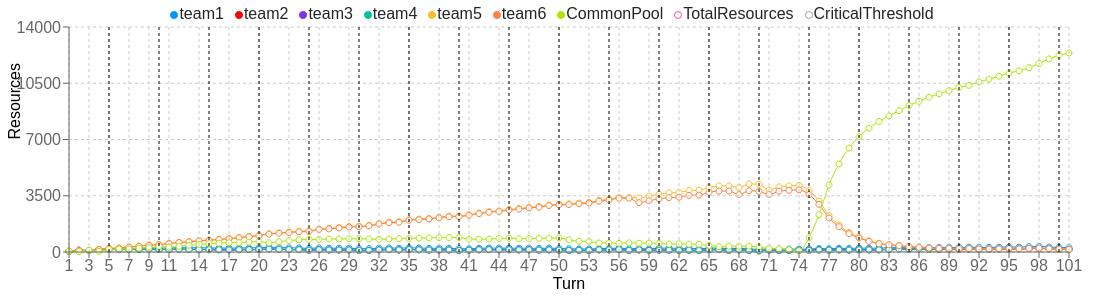
\includegraphics[width=0.9\textwidth]{09_team1_agentdesign/images/two_invaders}
\caption{Resource graph. Islands 5 and 6 are evading tax}
\label{fig:team1:two_invaders}
\end{figure}

\begin{figure}[H]
\centering
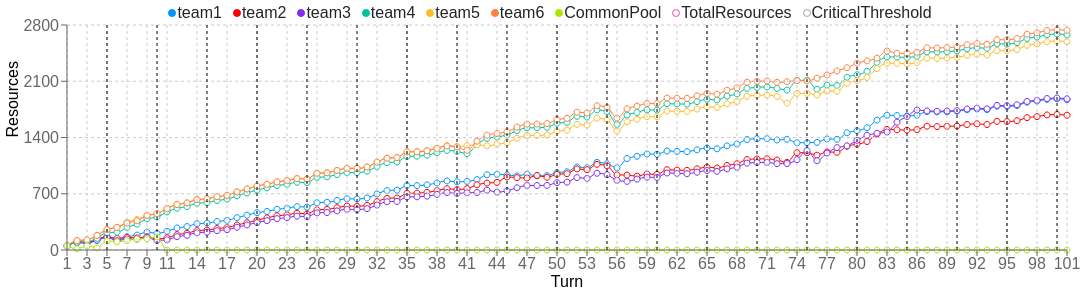
\includegraphics[width=0.9\textwidth]{09_team1_agentdesign/images/three_invaders}
\caption{Resource graph. Islands 4 to 6 are evading tax}
\label{fig:team1:three_invaders}
\end{figure}

Note here that collapse of IIGO (as in \autoref{fig:team1:three_invaders}, with three tax evaders) does not automatically imply collapse of the archipelago; the islands appeared to survive (and, in fact, thrive) even after the collapse of IIGO.\@ It was taken as an assumption that this was only due to the uniformity of strategies, and in the ``real'' simulation, with heterogeneous agents, collapse of IIGO would lead to collapse of the archipelago.



\section{Foraging}
Multiple foraging strategies were developed, initially by intuition and later by attempting to address the shortcomings of previous attempts. They were developed in order and aptly named:
\begin{itemize}
    \item Return on Investment (ROI)
    \item Regression
    \item Flip Forage
\end{itemize}


\subsection{Return on Investment (ROI) Foraging}%
\label{sec:forage-roi}

This first algorithm is based on repeating successful foraging behaviours in the past, whether those be by the agent herself or another agent.

For the first few turns (the exact amount is configurable) the agent will forage randomly.

The agent maintains a history of foraging decisions and outcomes, including those received from IIFO.\@ When it comes time to forage, this history is sorted by ROI, i.e.\ the ratio of profit to contribution. Decisions that resulted in a loss, had profit smaller than the living cost, or had a larger contribution than a (configurable) percentage of available resources, are filtered out.

\subsection{Regression Foraging}%
\label{sec:forage-regression}

This strategy tries to predict the ideal foraging decision, even if that exact decision was not made in the past. This is done using regression, which is used to find the decision with the highest expected reward.

The \emph{regression} strategy forages randomly in the initial turns and history is kept as in \nameref{sec:forage-roi}. To make a foraging decision, the history is split by foraged resource (fish or deer), and quadratic regression is performed on contribution versus reward for both resources. From this, a quadratic equation is formed. If the quadratic equation found is negative then the optimal contribution can be found by differentiation. If it is positive then a (large) value is chosen as contribution, as a higher contribution should simply lead to a higher reward.

\subsection{Flip Foraging}

This strategy chooses the least foraged resource from the last turn, according to IIFO-reported data. Contributed amount is proportional to the chosen resource's total ROI from last turn. This choice was made under the assumption that ROI is an indicator of the resource's ``condition''. If a resource only gives moderate rewards (proportionally to input) it means that it is probably over-used currently and as such agents should allow it to recover, by scaling down their foraging attempts or by switching foraging types.

\subsection{Comparison}

To compare the three strategies, simulations were run with six agents, two using \emph{ROI foraging}, two using \emph{regression foraging}, and two using \emph{flip foraging}. IIGO and IITO were also disabled in order to isolate the efficacy of foraging methods from other parts of the game. The simulation was run five times and the results averaged over the 5 games as well as the two agents following the same strategy.

\begin{figure}[H] 
\centering
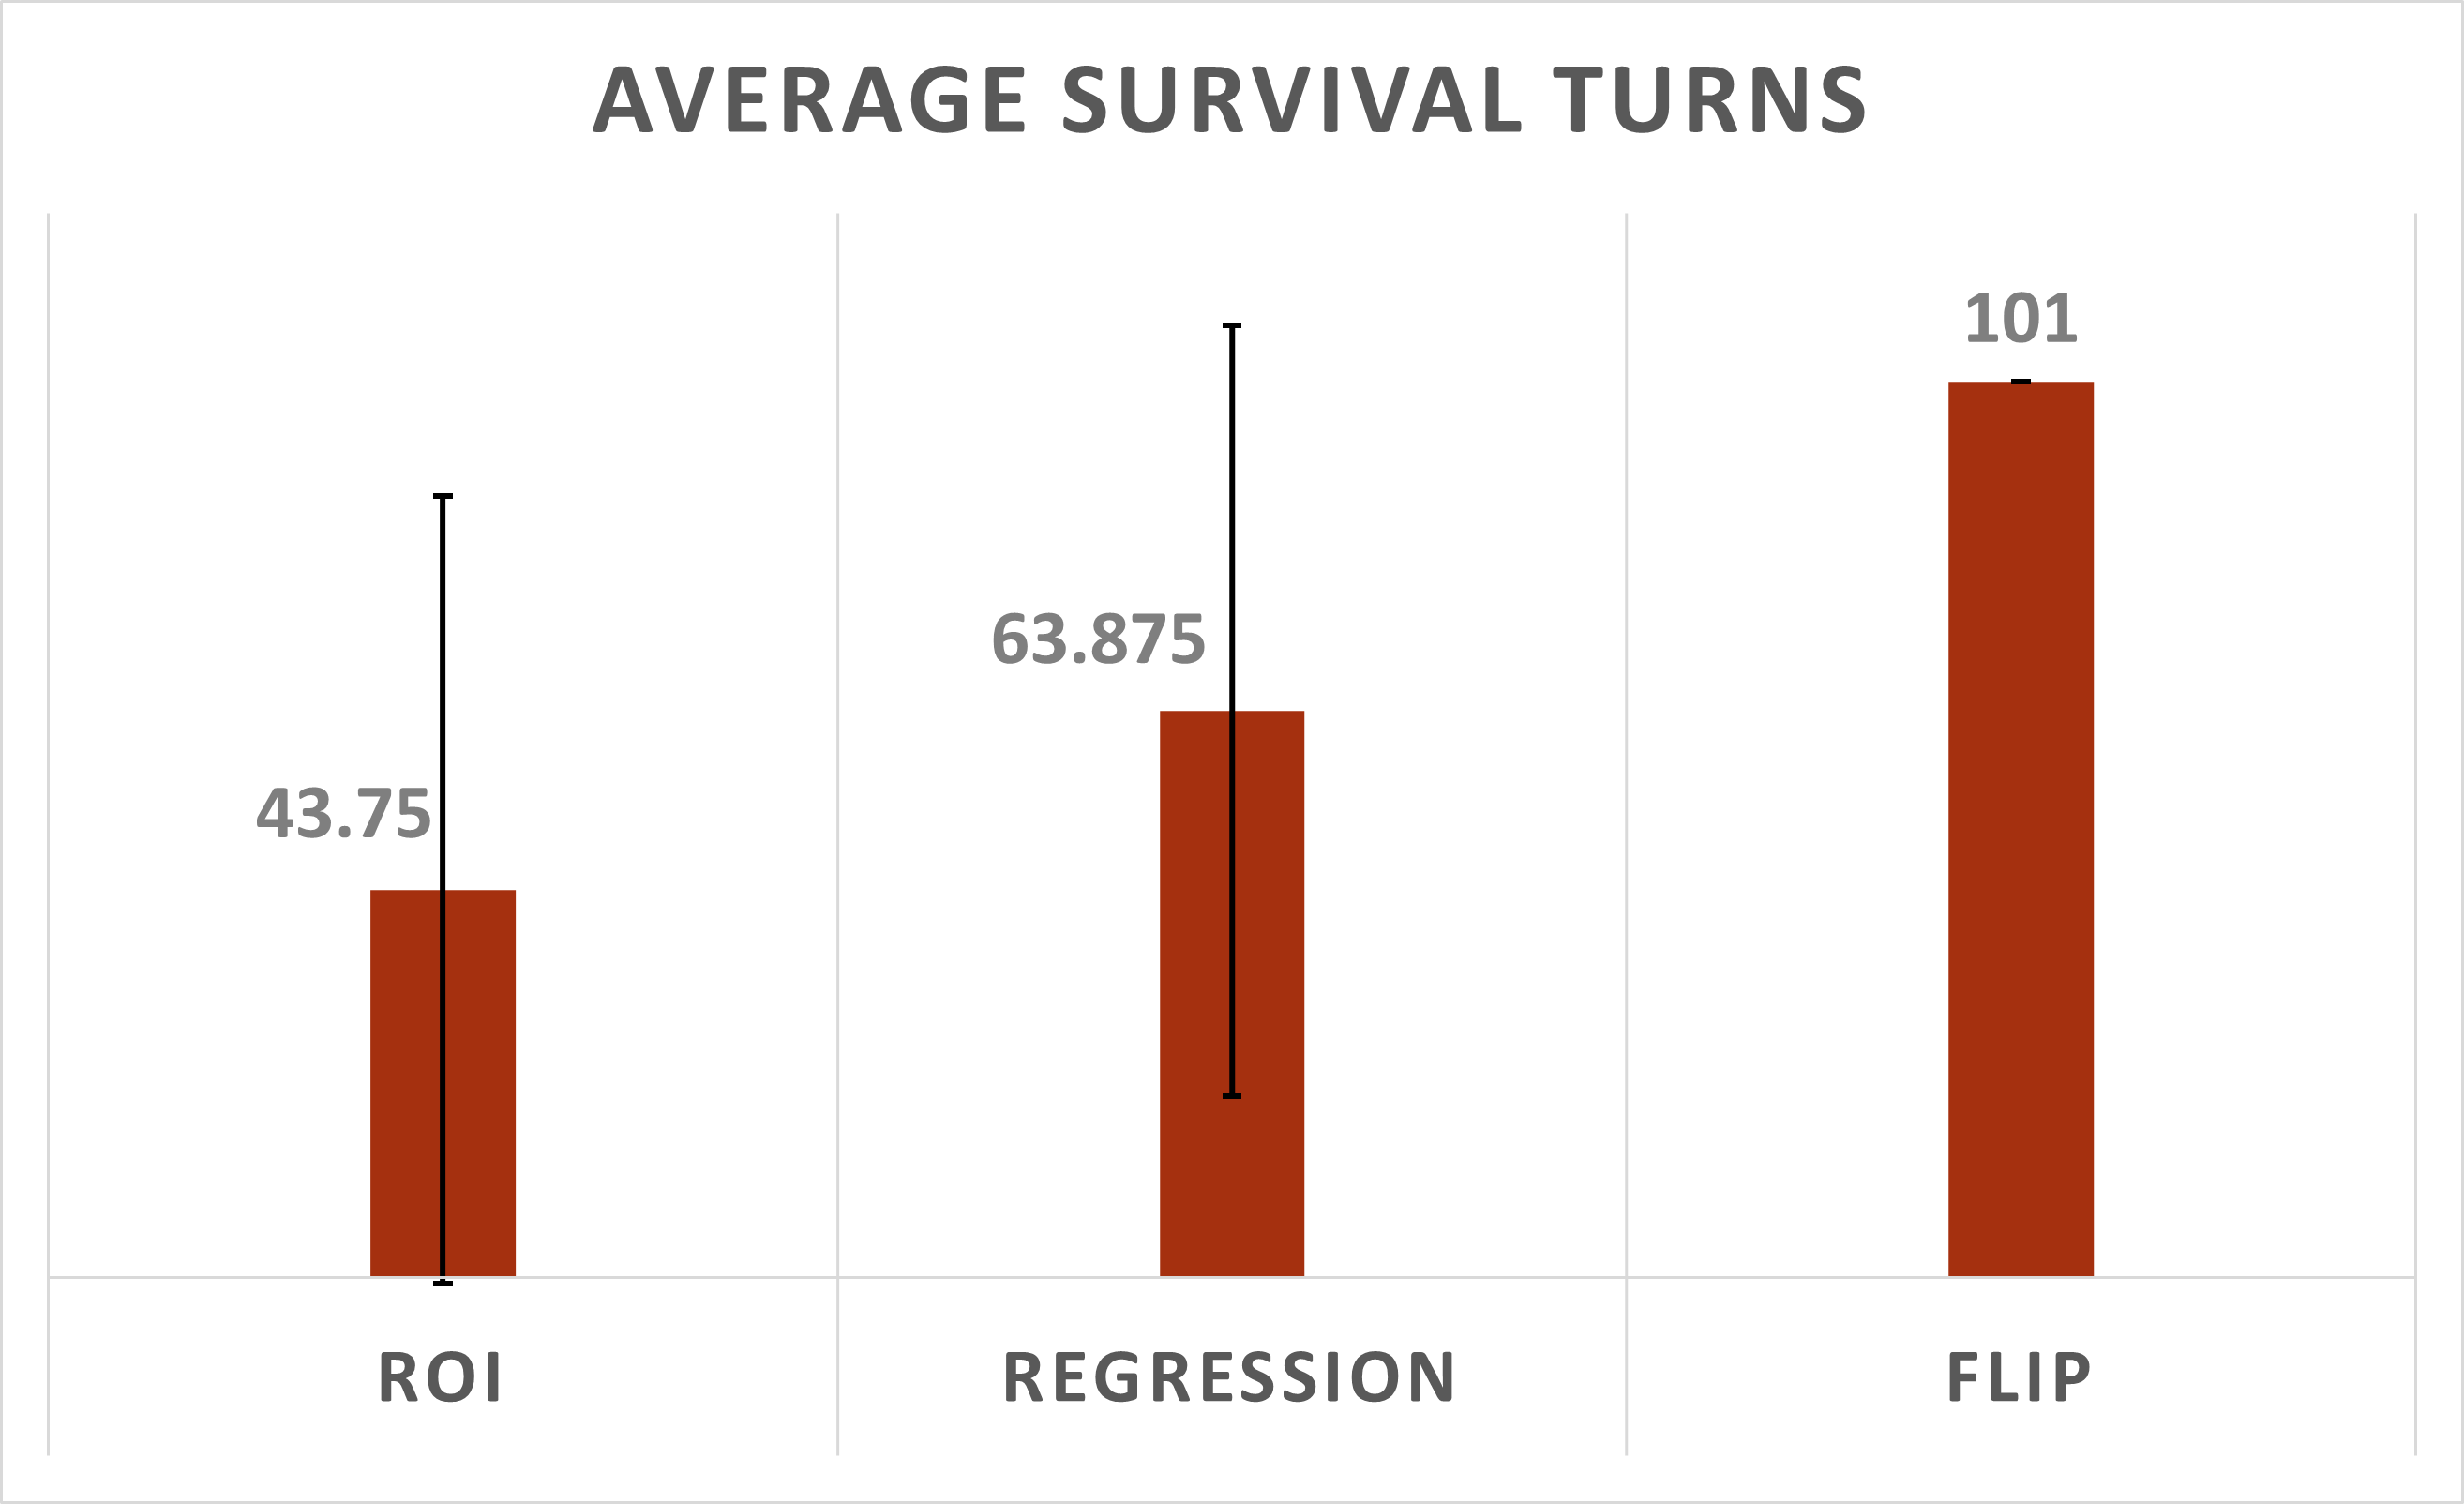
\includegraphics[width=0.6\textwidth]{09_team1_agentdesign/images/mean_survival_turns}
\caption{Mean survival turns for different strategies.}
\label{fig:team1:mean_survival}
\end{figure} 

\begin{figure}[H] 
\centering
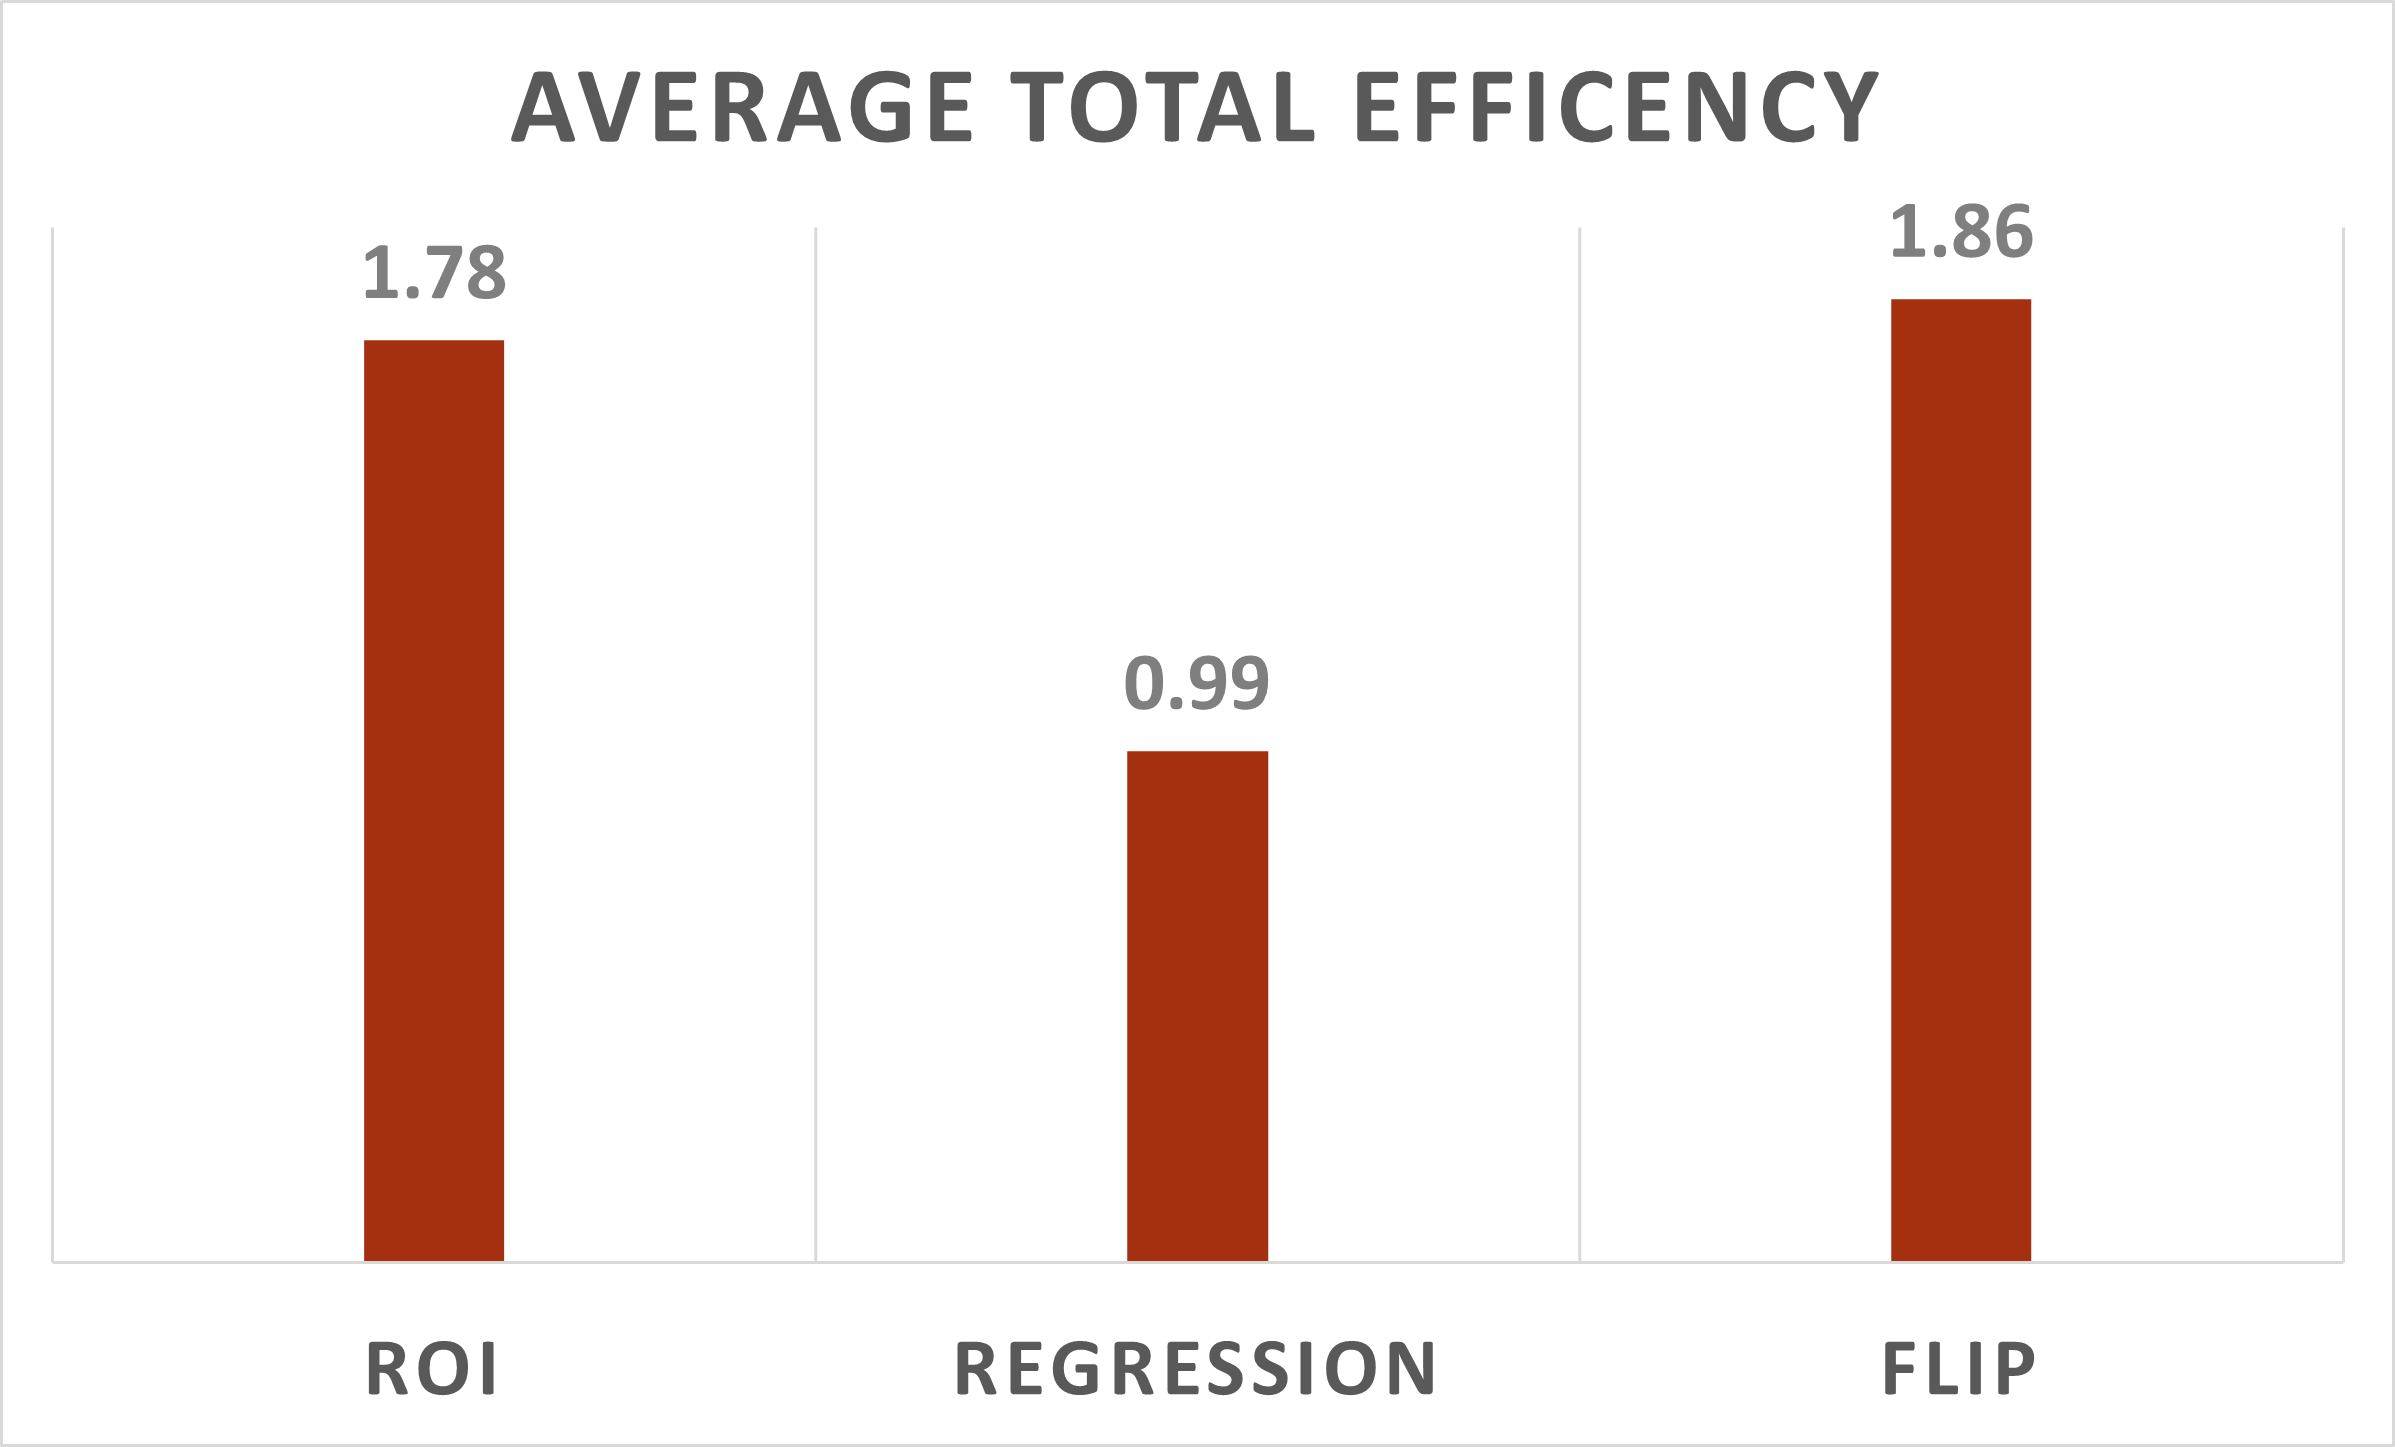
\includegraphics[width=0.6\textwidth]{09_team1_agentdesign/images/total_efficiency}
\caption{Average foraging efficiency}
\label{fig:team1:average_efficiency}
\end{figure} 

It is clear from \autoref{fig:team1:mean_survival} that the \emph{flip} foraging strategy dominates the other two in terms of overall effectiveness. However, it is interesting to note that, according to \autoref{fig:team1:average_efficiency}, the \emph{ROI} foraging method is almost as efficient as \emph{flip}, which raises the question of what causes the difference in their success. This difference could be attributed to one core issue with the \emph{ROI strategy}: ignoring the absolute value of rewards. The agent will happily settle for a profit of $11$ resources, if that was obtained with a contribution of $0.1$ resources (a profit of $110000\%$) over a profit $50$ resources for a contribution of $25$ (a measly $100\%$). This means that in the long run living costs overwhelm the \emph{ROI} agent. The \emph{flip} agent does not take expected profit into account and as such is unaffected by this.

\emph{Regression} appears to occupy a medium between \emph{flip} and \emph{ROI}, however it is much less consistent, as evidenced by the error bars in \autoref{fig:team1:mean_survival}, with \emph{regression} surviving for under 10 turns in some runs.

%%% Local Variables:
%%% mode: latex
%%% TeX-master: "../main"
%%% End:
